\documentclass[a4paper,10pt]{article}
\usepackage[utf8]{inputenc}
\usepackage[T1]{fontenc}
\usepackage[frenchb]{babel}
\usepackage{numprint}
\usepackage{graphicx}

%opening
\title{Apprentissage par des réseaux de neurones}
\author{E. Beghdadi, M. Marrakchi Benazzouz, T. Chabal, Y. Vanlaer, T. Giraudon}

\begin{document}

\maketitle

\begin{abstract}

\end{abstract}

\section{Introduction}
En 1963, l'Américain Donald Michie créé Menace, \textit{Machine Educable Noughts And Crosses Engine},
une machine capable de rivaliser avec des joueurs humains au jeu du Tic-Tac-Toe, plus connu en France sous le nom de morpion.
Pour réaliser cette prouesse technologique, il utilise alors la technique de \textit{l'apprentissage par renforcement}.
Celle-ci consiste à faire jouer la machine un grand nombre de fois contre un joueur réel et à apprendre de ces parties
en corrigeant sa stratégie au fur et à mesure. Cette réussite signe alors la naissance du machine learning tel que
nous le connaissons aujourd'hui. \\
Dans les années 1970-1980, beaucoup de progrès théoriques sont réalisés : on imagine ainsi un système
directement inspiré du vivant, le réseau de neurones. Celui-ci consiste en un agencement de couches de neurones successives,
appelés les \textit{layers}, indéxés par $L$. Plusieurs types de liaisons sont possibles; dans notre cas, chaque neurone du
\textit{layer} $L$ est relié à l'intégralité des neurones des \textit{layers} $L-1$ et $L+1$. Les premier et dernier \textit{layers}
jouent un rôle particulier : le premier correspond aux \textit{inputs}, les données d'entrée, et le dernier aux \textit{outputs},
les données de sortie. Les autres \textit{layers} sont qualifiés d'\textit{hidden layers}.
\\

\begin{figure}[h]
\centering
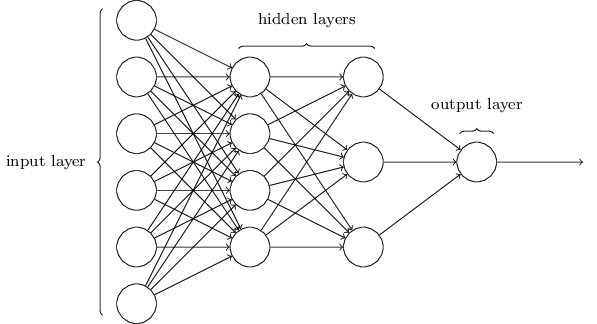
\includegraphics[scale = 0.4]{layers}
\caption{Structure du réseau de neurones}
 
\end{figure}



\section{Résultats}

\section{Discussion}

\section{Conclusion}


\end{document}
